\documentclass[10pt,twocolumn]{article}
\usepackage[letterpaper,margin=0.72in,columnsep=0.26in]{geometry}
\usepackage[T1]{fontenc}
\usepackage{mathptmx}
\usepackage[scaled=0.86]{helvet}
\usepackage{courier}
\usepackage{microtype}
\usepackage{amsmath,amssymb}
\usepackage{graphicx}
\usepackage{booktabs}
\usepackage{tabularx}
\usepackage{multirow}
\usepackage{makecell}
\usepackage[table]{xcolor}
\usepackage{tikz}
\usetikzlibrary{arrows.meta,positioning,fit,calc,shapes.misc}
\usepackage[font=small,labelfont=bf,skip=4pt]{caption}
\usepackage{subcaption}
\usepackage{enumitem}
\usepackage{float}
\usepackage[numbers,sort&compress]{natbib}
\usepackage{xurl}
\usepackage[colorlinks=true,linkcolor=blue!50!black,citecolor=green!35!black,urlcolor=blue!50!black]{hyperref}

\setlist{nosep,leftmargin=*}
\setlength{\textfloatsep}{8pt plus 2pt minus 2pt}
\setlength{\floatsep}{6pt plus 2pt minus 2pt}
\setlength{\dbltextfloatsep}{8pt plus 2pt minus 2pt}
\renewcommand{\arraystretch}{1.05}
\newcommand{\sys}{\textsf{unimem}}
\newcommand{\code}[1]{\texttt{\small #1}}
\newcommand{\para}[1]{\smallskip\noindent\textbf{#1}\ }
\newcommand{\yes}{\checkmark}
\newcommand{\RQ}[1]{\textbf{RQ#1}}
\definecolor{ours}{RGB}{232,240,250}
\definecolor{gw}{RGB}{31,78,121}

\title{\textbf{unimem: A Harness-Agnostic Memory Gateway for Coding Agents}}
\author{mapix\\ \small\url{https://github.com/mapix/unimem}}
\date{October 2026 \quad (software v0.5, commit \code{7c8742a})}

\begin{document}
\maketitle

\begin{abstract}
Every coding harness now ships its own memory: Claude Code has \code{CLAUDE.md} and auto memory, Codex has
\code{AGENTS.md} and its memories, and MCP- or hook-based memory servers must be wired into each harness separately.
The result is a set of silos: a correction given to one agent is unknown to the next. We argue that the model API is
the only integration point all harnesses share, and present \sys{}, a local gateway that sits behind the harness's
base URL and gives every harness one shared, project-scoped long-term memory without a plugin. \sys{} makes three
systems contributions: (i) \emph{cache-stable overlay replay}, which records every change it makes to a request
under a content anchor and re-applies it byte-for-byte, so every upstream request stays an exact byte-prefix extension of the previous one;
(ii) \emph{streaming interception and continuation} of its own tool calls across the Anthropic Messages, OpenAI
Responses and Chat Completions wire protocols, including mixed turns; and (iii) a \emph{memory-timing policy}
grounded in a survey of write/read triggers, with token budgets, a cross-turn de-dup ledger, compaction-aware
re-injection, tool-error recall and a pre-compaction flush. The memory engine follows Jev-Mem's System-One/System-Two
split with a pluggable typed decider. On a mock upstream, 1060/1060 interception assertions pass, 42/42 upstream
transitions are exact prefix extensions, and streaming adds 1.15\,ms p50 time-to-first-byte. On an out-of-sample
coding-memory suite, unified memory reaches cross-harness R@5 0.664 (0.671 with v0.5) where per-harness silos score 0.000. On the
test split of LongMemEval$_S$ and on LoCoMo, \sys{}'s ranker with a 118M-parameter e5 embedder is level with or
above BM25+e5 reciprocal-rank fusion (LoCoMo R@10 $+0.035$, 95\% CI $[+0.022,+0.047]$; LongMemEval turn R@10
$+0.025$, borderline). In a 120-request long-session simulation, the ledger removes all 128 duplicate injections
and the flush saves 5 of 6 planted facts before compaction (0 of 6 without it). We are explicit about what is
immature: all results are offline (heuristic decider, mock upstreams, LLM-authored synthetic suites), no
end-to-end QA or task-success metric was run, and the write-time injection screen caught only 1 of 7 held-out
injections.
\end{abstract}

%=====================================================================
\section{Introduction}
\label{sec:intro}

Long-term memory has become a standard feature of coding agents. Claude Code loads \code{CLAUDE.md} and an
agent-written auto memory at the start of each conversation and re-injects both after compaction~\cite{ccmemory,cccontext};
Codex extracts memories from idle chats in the background~\cite{codexmemories}; research systems such as
MemGPT~\cite{memgpt}, mem0~\cite{mem0}, Zep~\cite{zep}, A-MEM~\cite{amem} and Jev-Mem~\cite{jevmem2026} study how
memories should be written, linked, updated and retrieved. Yet a developer who uses more than one agent experiences
memory as a set of \emph{silos}. Each harness stores its notes in its own format and location, none can read the
others', and most do not separate facts ``about me'' from facts ``about this repository''. Memory servers exposed
over MCP or harness hooks can share a store, but each must be configured per harness, and they depend on the agent
choosing to call them.

\para{Thesis.} Memory belongs to the user, not to the tool. If memory is to be shared, it must live outside every
harness. Among all the places it could live, the model API is the only one every harness is guaranteed to use, and
every harness lets the user change its base URL. A gateway at that point needs zero per-harness integration. Because
it runs on the user's machine, it can also read the working directory the harness mentions and resolve the git
project deterministically.

The gateway position is attractive but unforgiving. A gateway that edits requests can silently break the provider's
prompt cache, which is a prefix match. Tools it exposes must never leak into a harness that does not know them,
which requires rewriting streamed responses in flight. Memory it injects competes with the task for context, and a
naive policy grows without bound until the harness compacts---after which the memory is gone. This paper describes
how \sys{} handles each of these and measures how well it does.

\para{Contributions.}
\begin{enumerate}
\item \textbf{A harness-agnostic memory gateway} with \emph{cache-stable overlay replay}: every modification is
  stored under a content anchor derived from what the harness echoes back, scoped by session, and replayed
  byte-identically, which keeps every upstream request an exact prefix extension of the previous one (\S\ref{sec:overlay}).
\item \textbf{Streaming interception and continuation} across three wire protocols (Anthropic Messages, OpenAI
  Responses, Chat Completions), including turns that mix gateway tools with harness tools (\S\ref{sec:intercept}).
\item \textbf{A memory-timing design grounded in a survey} of when frontier systems write and read memory: token
  budgets derived from the model's window, a cross-turn de-dup ledger, compaction detection and re-injection,
  tool-error-triggered recall and a pre-compaction flush (\S\ref{sec:timing}).
\item \textbf{A Jev-Mem-style engine} in which a pluggable System-One decider answers batched typed questions,
  each with a code-computed prior, and recall is a calibrated hybrid ranker with an adaptive cut-off (\S\ref{sec:engine}).
\item \textbf{An evaluation} on the standard LongMemEval$_S$~\cite{longmemeval} and LoCoMo~\cite{locomo} retrieval
  tasks with a dev/test split and bootstrap CIs, plus new coding-agent memory suites with explicit in-sample/out-of-sample
  discipline, gateway micro-benchmarks and a long-session simulation (\S\ref{sec:eval}). We report negative results,
  including a version that overfit its own benchmark (\S\ref{sec:lessons}), and a long list of immature aspects (\S\ref{sec:limits}).
\item \textbf{An open-source Rust implementation}~\cite{unimemrepo}: one binary with an embedded SQLite store, an
  MCP endpoint, a CLI and a local web UI.
\end{enumerate}

%=====================================================================
\section{Background and Related Work}
\label{sec:related}

\para{Harness-native memory.} Claude Code loads \code{CLAUDE.md} (user-written) and auto memory (written by the
agent ``based on your corrections and preferences'') at session start; only the first 200 lines or 25\,KB of the
\code{MEMORY.md} index load, and topic files are read on demand~\cite{ccmemory}. Its hooks (\code{SessionStart},
\code{UserPromptSubmit}, \code{PostToolUse}, \code{PreCompact}, \code{SessionEnd}) let scripts add context, with
\code{additionalContext} capped at 10,000 characters~\cite{cchooks}. After compaction, hook-added context is
summarized with the rest of the conversation, and only \code{CLAUDE.md}, auto memory and \code{SessionStart(compact)}
output are re-injected~\cite{cccontext}. Codex memories are off by default and are extracted in the background from
idle chats, skipped when the rate-limit remaining percentage is low~\cite{codexmemories}. All of these are bound to
one harness's format and directory. \sys{} does not replace them; it adds a layer shared across harnesses.

\para{Agent memory systems.} mem0 extracts candidate facts per message pair and updates the store with
ADD/UPDATE/DELETE/NOOP operations chosen by an LLM~\cite{mem0}. MemGPT lets the model manage its own memory through
function calls and inserts a memory-pressure warning at about 70\% of the window~\cite{memgpt}. Sleep-time
compute~\cite{sleeptime} and Letta's ``dreaming''~\cite{lettadocs} move consolidation off the hot path, triggered every
$N$ steps or on compaction. Zep/Graphiti stores bi-temporal edges and invalidates contradicted ones instead of deleting
them~\cite{zep}. LangMem separates hot-path from debounced background formation~\cite{langmem}. A-MEM links each new
note to related notes and evolves old ones~\cite{amem}. MemoryOS promotes memories across three tiers by
heat~\cite{memoryos}. Generative Agents reflect when summed importance exceeds 150~\cite{genagents}, and MemoryBank
applies Ebbinghaus-style decay~\cite{memorybank}. Jev-Mem~\cite{jevmem2026} delegates the many small typed
decisions of a memory system (typing, relations, routing, budgets, scoring, stopping) to a fast probabilistic
``System One'' model and reserves the large model (``System Two'') for reasoning; its reference implementation
gates per-prompt recall with one System-One call and consolidates every 20 writes~\cite{jevmemrepo}. Coding-agent
tools such as memsearch~\cite{memsearch} and OpenWolf~\cite{openwolf} attach to harness hooks. \sys{}'s engine follows
Jev-Mem's split; its contribution is \emph{where} memory runs (the API boundary) and \emph{when} it is written and read.

\para{Benchmarks.} LongMemEval~\cite{longmemeval} decomposes long-term memory into indexing, retrieval and reading,
and reports that long-context models lose about 30\% accuracy on sustained interaction, so keeping everything in
context is no substitute. LoCoMo~\cite{locomo} evaluates very long multi-session dialogues. Both are chat benchmarks;
we use their retrieval tasks and add coding-specific suites (\S\ref{sec:eval}). Recent work warns that relevance
ranking does not close evidence gaps~\cite{relevancesufficiency}, that shared memory can expose credentials across
owners~\cite{whosecredential}, that contracted memories ``quietly answer wrong'' once facts change~\cite{manysteps},
and that a remembered proposal must not become an authorization~\cite{groundingawareness}; each maps onto a
limitation we observe.

\para{Memory-first proxies.} BladeX~\cite{bladex} (a self-hosted memory-first proxy for agents) and
NautGate~\cite{nautgate} (a memory-aware LLM gateway) also place memory at the model API. Both predate this work
(their repositories were created in May 2026); \sys{} was designed independently from first principles. We have not compared against them
experimentally, and differences in mechanism (overlay replay, interception, scope decisions) are not established
by this paper.

\para{Timing survey.} Table~\ref{tab:survey} condenses our survey (\code{docs/REVIEW.md}) of when systems write and
read memory. Every row is drawn from a source fetched for that review; entries we could not verify are marked n/d.
The survey motivates the taxonomy of \S\ref{sec:timing}.

\begin{table*}[t]
\centering\scriptsize
\caption{When frontier systems write and read memory (condensed from the design review; all sources fetched October 2026).
n/d = not documented in the fetched source. The last row is this work.}
\label{tab:survey}
\setlength{\tabcolsep}{3.5pt}
\begin{tabularx}{\textwidth}{@{}l>{\raggedright\arraybackslash}X>{\raggedright\arraybackslash}p{2.3cm}>{\raggedright\arraybackslash}X>{\raggedright\arraybackslash}p{2.9cm}>{\raggedright\arraybackslash}p{2.6cm}@{}}
\toprule
System & Write trigger(s) & Who extracts & Read trigger(s) & Budget / placement & Update / forget \\
\midrule
Claude Code \code{CLAUDE.md}~\cite{ccmemory} & explicit user edit, \code{/init} & user (agent on request) & session start; nested files on access; re-injected after compaction & target $<$200 lines & manual \\
Claude Code auto memory~\cite{ccmemory} & hot path: agent writes files mid-session & in-loop model & session start (index 200 lines/25\,KB); topic files on demand; re-injected after compaction & hard index cap with reminders & agent edits/merges \\
Claude Code hooks~\cite{cchooks} & any lifecycle event & hook script & SessionStart, UserPromptSubmit, PostToolUse & $\le$10,000 chars per hook & n/a \\
Codex memories~\cite{codexmemories} & idle-based background extraction; skipped at low rate limit & extract + consolidation models & future sessions & n/d & background consolidation \\
mem0~\cite{mem0} & every message pair & LLM extractor & per query & top-$k$ & ADD/UPDATE/ DELETE/NOOP \\
MemGPT~\cite{memgpt} & agent function calls; pressure warning at $\sim$70\% & in-loop model & agent-initiated search; working context & OS-style tiers & self-editing \\
Letta dreaming~\cite{lettadocs} & every $N$ steps or on compaction & sleep-time subagents & memory blocks in context & block sizes & background rewrite \\
Zep/Graphiti~\cite{zep} & every ingested episode & LLM pipeline & per query search + rerank & top-$k$ & bi-temporal invalidation \\
LangMem~\cite{langmem} & hot-path tools or debounced background & in-loop or background & tool or prefetch & app-defined & extract, update, consolidate \\
A-MEM~\cite{amem} & every add: link + evolve & LLM & n/d & top-$k$ & evolution updates \\
MemoryOS~\cite{memoryos} & STM$\to$MTM FIFO; heat $>\tau$ & system & each response, all tiers & top-$m$/top-$k$ & heat-based replacement \\
Generative Agents~\cite{genagents} & reflection when $\Sigma$importance $>150$ & LLM & each action & top-$k$ & none \\
MemoryBank~\cite{memorybank} & each interaction & LLM summary & each turn & top-$k$ & Ebbinghaus decay \\
jevmem~\cite{jevmemrepo} & hot-path tool; auto-capture; consolidation every 20 writes & in-loop + System One & SessionStart; per-prompt gate + subject filter & 1--3 notes per recall & supersede/duplicate flags \\
memsearch~\cite{memsearch} & Stop hook every turn & small model & before first step when useful & 3-level progressive & journals + summaries \\
OpenWolf~\cite{openwolf} & hook checkpoints & hooks & restore after compaction/restart & n/d & archive \\
\rowcolor{ours} \sys{} v0.4+ & hot-path tool (default); idle/session-end distiller (off); pre-compaction flush & in-loop model; optional cheap model & preamble on first prompt and after compaction; gated passive recall per prompt; tool-error recall; agent tool & per-turn, preamble, tool and per-session token budgets & write-time supersede/duplicate; forget tool \\
\bottomrule
\end{tabularx}
\end{table*}

%=====================================================================
\section{Design}
\label{sec:design}

\subsection{First principles}
\label{sec:principles}
We derived \sys{} from seven constraints rather than from an existing product.
\textbf{P1} Memory belongs to the person, so it must sit outside, and be shared by, all harnesses.
\textbf{P2} The model API is the only universal integration point; every harness supports a custom base URL.
\textbf{P3} A local gateway can see the file system, so project identity has deterministic hard signals; only
semantics (what the project does, whether a note is global) needs a model.
\textbf{P4} The smartest model is already in the loop (System Two); give it tools instead of paying another large
model to summarize.
\textbf{P5} Frequent small decisions (store this? which scope? conflicts with which note? does this prompt need
memory? is the evidence sufficient?) go to a fast typed System-One decider with thresholds in code.
\textbf{P6} The user must not pay for memory with cache misses: any injection is either byte-stable for the whole
session or appended at the tail and replayed verbatim afterwards.
\textbf{P7} Failure must be transparent: any memory-layer error degrades to pure pass-through.

\subsection{Architecture and turn classification}
\label{sec:arch}

\begin{figure*}[t]
\centering
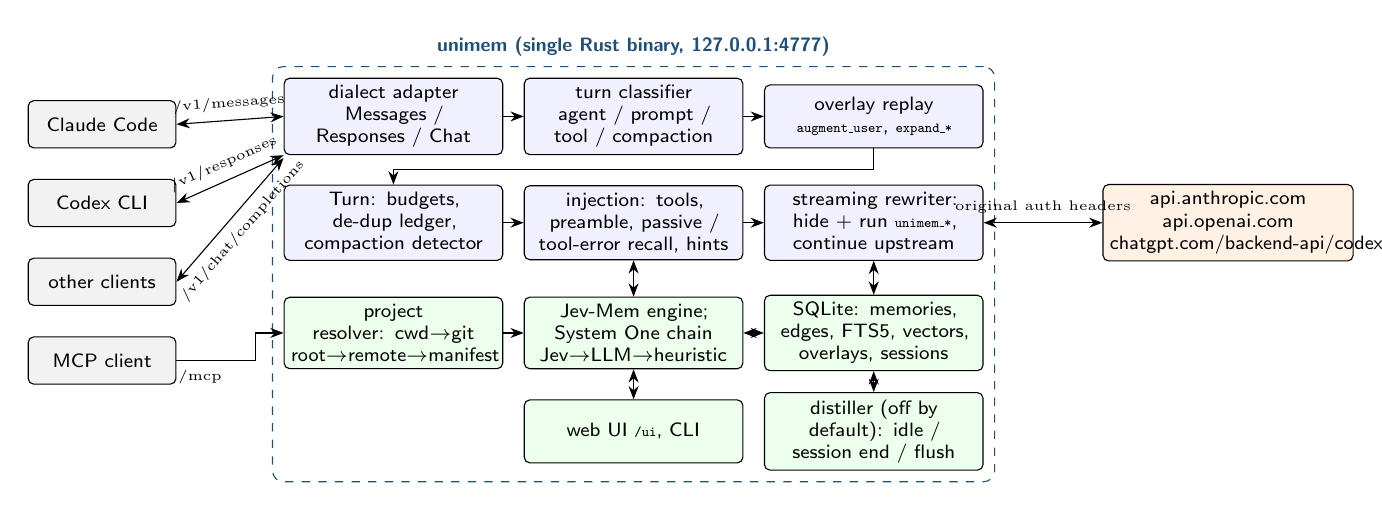
\begin{tikzpicture}[
  font=\sffamily\scriptsize, >=Stealth,
  box/.style={draw, rounded corners=2pt, align=center, inner sep=2.5pt, text width=2.6cm, minimum height=0.8cm,
    execute at begin node={\hyphenpenalty=10000\exhyphenpenalty=10000}},
  hb/.style={box, fill=gray!10, text width=1.7cm, minimum height=0.6cm},
  gb/.style={box, fill=blue!6},
  eb/.style={box, fill=green!7},
  ub/.style={box, fill=orange!10, text width=3.0cm}]
\newcommand{\tc}[1]{{\ttfamily\tiny #1}}
\node[hb] (cc) at (0,1.5) {Claude Code};
\node[hb] (cx) at (0,0.5) {Codex CLI};
\node[hb] (ot) at (0,-0.5) {other clients};
\node[hb] (mcp) at (0,-1.5) {MCP client};
\node[gb] (dia) at (3.7,1.6) {dialect adapter\\Messages / Responses / Chat};
\node[gb] (tc)  at (6.75,1.6) {turn classifier\\agent / prompt / tool / compaction};
\node[gb] (ov)  at (9.8,1.6) {overlay replay\\\tc{augment\_user}, \tc{expand\_*}};
\node[gb] (bud) at (3.7,0.25) {Turn: budgets, de-dup ledger, compaction detector};
\node[gb] (inj) at (6.75,0.25) {injection: tools, preamble, passive / tool-error recall, hints};
\node[gb] (rw)  at (9.8,0.25) {streaming rewriter: hide + run \tc{unimem\_*}, continue upstream};
\node[eb] (pj)  at (3.7,-1.15) {project resolver: cwd$\to$git root$\to$remote$\to$manifest};
\node[eb] (eng) at (6.75,-1.15) {Jev-Mem engine; System One chain Jev$\to$LLM$\to$heuristic};
\node[eb] (st)  at (9.8,-1.15) {SQLite: memories, edges, FTS5, vectors, overlays, sessions};
\node[eb] (ui)  at (6.75,-2.4) {web UI \tc{/ui}, CLI};
\node[eb] (ds)  at (9.8,-2.4) {distiller (off by default): idle / session end / flush};
\node[ub] (up) at (14.3,0.25) {api.anthropic.com\\api.openai.com\\chatgpt.com/backend-api/codex};
\node[draw=gw, dashed, rounded corners=4pt, inner sep=4pt, fit=(dia)(ov)(ds)(pj),
  label={[gw,font=\sffamily\scriptsize\bfseries]above:unimem (single Rust binary, 127.0.0.1:4777)}] (gwbox) {};
\draw[<->] (cc.east) -- node[above,font=\tiny,sloped]{/v1/messages} (dia.west);
\draw[<->] (cx.east) -- node[above,font=\tiny,sloped]{/v1/responses} (dia.south west);
\draw[<->] (ot.east) -- node[below,font=\tiny,sloped]{/v1/chat/completions} ([yshift=-1pt]dia.south west);
\draw[->] (mcp.east) -- node[below,font=\tiny,pos=0.3]{/mcp} ++(1.0,0) |- (pj.west);
\draw[->] (dia) -- (tc); \draw[->] (tc) -- (ov);
\draw[->] (ov.south) -- ++(0,-0.27) -| (bud.north);
\draw[->] (bud) -- (inj); \draw[->] (inj) -- (rw);
\draw[<->] (rw.east) -- node[above,font=\tiny]{original auth headers} (up.west);
\draw[<->] (inj) -- (eng); \draw[<->] (rw.south) -- (st.north); \draw[<->] (eng) -- (st); \draw[->] (pj) -- (eng);
\draw[<->] (ds) -- (st); \draw[<->] (ui) -- (eng);
\end{tikzpicture}
\caption{Architecture. Harnesses point their base URL at \sys{}; the gateway classifies each request, replays its
overlays, applies the timing policy, injects tools and memory, and rewrites the upstream stream so that
\code{unimem\_*} tool calls are executed inside the gateway. All state lives in one SQLite file.}
\label{fig:arch}
\end{figure*}

Figure~\ref{fig:arch} shows the architecture. Not every request should receive memory: harnesses issue many helper
requests (title generation, command-prefix checks, quota probes, their own compaction summaries). \sys{} therefore
classifies each request:
\begin{itemize}
\item \textbf{agent turn}: the request carries \code{tools}. \sys{} appends its four tools (\code{unimem\_recall},
  \code{unimem\_remember}, \code{unimem\_forget}, \code{unimem\_project}) and replays overlays;
\item \textbf{prompt turn}: an agent turn whose last message is new user text; it additionally gets the session
  preamble (if not live) and gated passive recall;
\item \textbf{tool turn}: the last message is a tool result (Anthropic \code{tool\_result}, Responses
  \code{*\_output} items, Chat \code{role:\,tool}); it gets recall only if the output looks like an error (\S\ref{sec:timing});
\item \textbf{compaction request}: the harness asks the model to summarize the conversation (matched by its
  instruction wording); it is passed through unmodified---no tools, no recall, no episode;
\item \code{count\_tokens}: our tools are appended and overlays replayed, so the harness estimates the request that is
  actually sent;
\item anything else (no tools, model lists): pure pass-through.
\end{itemize}
The system prompt is never modified, because some subscription authentication validates its prefix, and tools are
appended after the harness's own. Upstream routing preserves the original authentication headers; the Responses
dialect routes to \code{chatgpt.com/backend-api/codex} when the request carries a \code{chatgpt-account-id}.

\subsection{Cache-stable overlay replay}
\label{sec:overlay}

Provider prompt caches match on a byte prefix of the serialized request (tools, then system, then messages). Any
change the gateway makes therefore has to be reproduced exactly on every later request of the conversation, even
though the harness never sees it. We formalize the mechanism.

\para{Model.} A conversation in session $s$ is a sequence of harness-visible messages $h=(m_1,\dots,m_n)$. The harness
sends $h$ on every request, extending it monotonically between compactions. The gateway keeps an append-only
overlay store $\mathcal{O}$ mapping anchors to payloads. A content key $\kappa(m)$ hashes what the harness echoes back
verbatim: user text and \code{tool\_result} ids for user messages; trimmed \code{text} and \code{tool\_use} ids for
assistant messages, ignoring thinking blocks, signatures, citations and \code{cache\_control}. Two overlay kinds
exist:
\begin{align*}
a^{\text{aug}}_i &= H(\text{``aug''},\, s,\, \kappa(m_{i-1}),\, \kappa(m_i)),\\
a^{\text{exp}}_i &= H(\text{``exp''},\, s,\, \kappa(m_{i-1}),\, H(\text{``vis''}, \kappa(m_i))).
\end{align*}
An \code{augment\_user} payload is text appended to user message $m_i$ (preamble, passive recall, tool-error recall,
hints). An \code{expand\_assistant} payload replaces the merged assistant message $m_i$ the harness saw with the true
upstream sequence $\langle$assistant(with \code{unimem\_*} calls), user(\code{tool\_result}), assistant(continuation)$\rangle$,
plus any trailing results to prepend to $m_{i+1}$ in mixed turns. The Responses dialect anchors runs of hidden items
before or after adjacent visible output items (keyed by \code{call\_id}, reasoning \code{encrypted\_content} hash, or
message text). The upstream request is $R(h)=\rho(m_1)\cdots\rho(m_n)$ where $\rho(m_i)$ applies whichever overlays
match $m_i$, plus the fixed tool definitions. New augmentation is only ever added to the \emph{last} message $m_n$ and is
stored in $\mathcal{O}$ before the request is sent upstream; an empty payload records ``already processed'' so retries
are idempotent.

\para{Invariants.}
(\emph{I1, prefix stability}) If $h$ is a prefix of $h'$ and no compaction occurred, then $R(h)$ is a byte prefix of
$R(h')$: $\rho$ is deterministic, $\mathcal{O}$ is append-only, every anchor depends only on $s$ and the message pair,
and tool definitions are constant. Continuation rounds within one visible turn are themselves prefix extensions.
(\emph{I2, session isolation}) Because $s$ is part of every anchor, a conversation never replays another
conversation's hidden rounds, even when both share a prompt and a deterministic reply.
(\emph{I3, graceful degradation}) If an anchor does not match (compaction, edited history, trimmed blocks), the overlay
is skipped and the request remains well-formed; only that memory context is lost.
(\emph{I4, invisibility}) No \code{unimem\_*} block and no \code{<unimem\ldots>} text is ever returned to the harness.
We test I1, I2 and I4 directly in \S\ref{sec:rq3}. I1 is the reason passive recall is appended to the \emph{current}
user message (the tail) rather than to the system prompt; \S\ref{sec:rq3} quantifies what the naive alternatives cost.

\subsection{Streaming interception and continuation}
\label{sec:intercept}

The harness does not know \sys{}'s tools, so their calls must never reach it. Figure~\ref{fig:intercept} shows the
streaming rewriter. It forwards upstream SSE events while maintaining a block (or item) index map. A content block
that opens a \code{unimem\_*} tool call is buffered, and later blocks are renumbered so the harness sees contiguous
indices. When the round ends with \code{stop\_reason=tool\_use}:
\begin{itemize}
\item \textbf{only our tools}: \code{message\_delta}/\code{message\_stop} are swallowed, the tools run inside the
  gateway, and the assistant message plus \code{tool\_result} are appended to the request and sent upstream again. The
  new stream's \code{message\_start} is skipped and its indices are offset, so the harness sees one continuous
  message. An \code{expand\_assistant} overlay is recorded. At most \code{max\_continuations}\,=\,6 rounds run per
  visible response.
\item \textbf{mixed} (our tools and the harness's, e.g.\ \code{Bash}): the harness's calls are delivered normally; ours
  run in the gateway and their results are stored as an overlay that re-inserts our \code{tool\_use} into the assistant
  message and prepends our \code{tool\_result} to the next user message.
\end{itemize}
The Responses dialect applies the same machine to output items, renumbering \code{output\_index} and
\code{sequence\_number} and emitting a single \code{response.completed} whose \code{output} holds only visible items. The
Chat dialect buffers \code{tool\_calls} by index and joins later rounds' text with a blank line. JSON
(non-streaming) responses use the same logic without the event pump.

\para{Honest usage.} A merged response reports the \emph{last} round's \code{input\_tokens} and \code{cache\_*}
fields (the true context size, which harnesses use to decide when to compact) and the \emph{sum} of output tokens.
True totals over all rounds are returned in an \code{x-unimem-usage} header (JSON, with \code{rounds}) or a trailing
SSE comment, and logged. Earlier versions summed every field, which could overstate context by the number of rounds.

\begin{figure}[t]
\centering
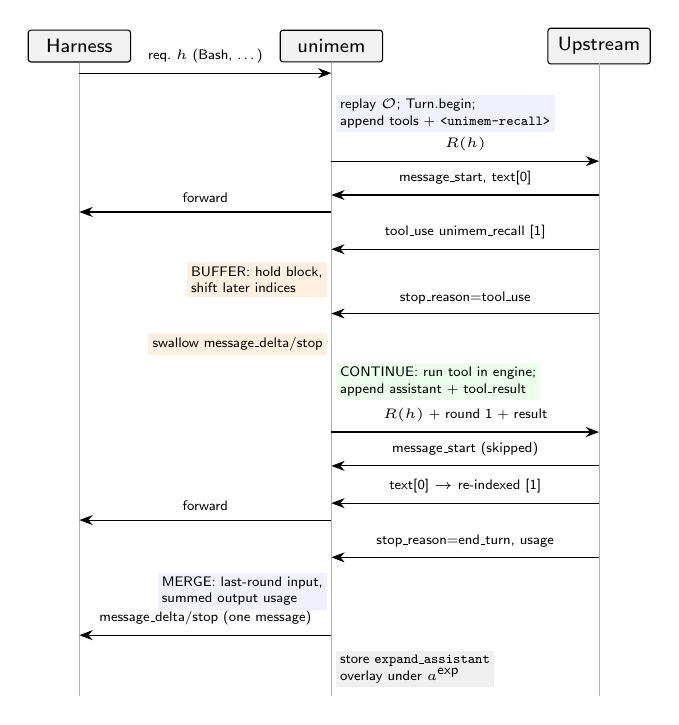
\begin{tikzpicture}[font=\sffamily\tiny, >=Stealth, x=1cm, y=0.43cm,
  note/.style={align=left,inner sep=1.5pt}]
\renewcommand{\code}[1]{{\ttfamily #1}}
\def\H{0} \def\G{3.2} \def\U{6.6}
\foreach \x/\n in {\H/Harness, \G/unimem, \U/Upstream}{
  \node[draw, fill=gray!10, rounded corners=1pt, minimum width=1.3cm, font=\sffamily\scriptsize] at (\x,0.8) {\n};
  \draw[gray!60] (\x,0.3) -- (\x,-18.4);}
\draw[->] (\H,0) -- node[above]{req.\ $h$ (Bash, \ldots)} (\G,0);
\node[note,right,fill=blue!6] at (\G+0.05,-1.2) {replay $\mathcal{O}$; Turn.begin;\\append tools + \code{<unimem-recall>}};
\draw[->] (\G,-2.6) -- node[above]{$R(h)$} (\U,-2.6);
\draw[->] (\U,-3.6) -- node[above]{message\_start, text[0]} (\G,-3.6);
\draw[->] (\G,-4.1) -- node[above]{forward} (\H,-4.1);
\draw[->] (\U,-5.2) -- node[above]{tool\_use unimem\_recall [1]} (\G,-5.2);
\node[note,left,fill=orange!12] at (\G-0.05,-6.1) {BUFFER: hold block,\\shift later indices};
\draw[->] (\U,-7.1) -- node[above]{stop\_reason=tool\_use} (\G,-7.1);
\node[note,left,fill=orange!12] at (\G-0.05,-8.0) {swallow message\_delta/stop};
\node[note,right,fill=green!8] at (\G+0.05,-9.1) {CONTINUE: run tool in engine;\\append assistant + tool\_result};
\draw[->] (\G,-10.6) -- node[above]{$R(h)$ + round 1 + result} (\U,-10.6);
\draw[->] (\U,-11.6) -- node[above]{message\_start (skipped)} (\G,-11.6);
\draw[->] (\U,-12.7) -- node[above]{text[0] $\to$ re-indexed [1]} (\G,-12.7);
\draw[->] (\G,-13.2) -- node[above]{forward} (\H,-13.2);
\draw[->] (\U,-14.3) -- node[above]{stop\_reason=end\_turn, usage} (\G,-14.3);
\node[note,left,fill=blue!6] at (\G-0.05,-15.3) {MERGE: last-round input,\\summed output usage};
\draw[->] (\G,-16.6) -- node[above]{message\_delta/stop (one message)} (\H,-16.6);
\node[note,right,fill=gray!12] at (\G+0.05,-17.6) {store \code{expand\_assistant}\\overlay under $a^{\text{exp}}$};
\end{tikzpicture}
\caption{Interception of a gateway-only tool round (Anthropic dialect). The harness receives one well-formed message with
contiguous block indices; the hidden round is stored and replayed on later requests.}
\label{fig:intercept}
\end{figure}

\subsection{Memory timing: when to write and when to read}
\label{sec:timing}

Our survey (Table~\ref{tab:survey}) yields seven write triggers and five read triggers (Table~\ref{tab:taxonomy}).
\sys{} v0.3 implemented only W1, an optional W3, R1, R2 and R3; the design review found that its injection was
unbounded, that compaction silently disabled memory, and that usage was over-reported. v0.4 adds W4, R4 and R5 and
bounds everything with budgets. Each agent request passes through \code{Turn::begin}, which loads per-conversation
state keyed by \code{session\#}hash(first user message), so subagents that share a session id but start differently
get their own preamble and ledger.

\begin{table}[t]
\centering\scriptsize
\caption{Taxonomy of memory triggers and which ones \sys{} implements (version added).}
\label{tab:taxonomy}
\setlength{\tabcolsep}{3pt}
\begin{tabularx}{\columnwidth}{@{}l>{\raggedright\arraybackslash}X>{\raggedright\arraybackslash}p{2.35cm}@{}}
\toprule
& Trigger (examples) & \sys{} \\
\midrule
W1 & hot-path tool call by agent (auto memory, MemGPT) & \yes\ remember tool (v0.1) \\
W2 & per-turn extraction (mem0, memsearch) & -- \\
W3 & idle / session-end batch (Codex, LangMem) & \yes\ distiller, off by default (v0.1; session end v0.4) \\
W4 & pre-compaction flush (MemGPT 70\%, Letta) & \yes\ at 70\% of window (v0.4) \\
W5 & importance-threshold reflection (Gen.\ Agents) & partial: correction importance $+3$ only \\
W6 & sleep-time consolidation (Letta, jevmem) & -- \\
W7 & explicit user command & via W1 \\
\midrule
R1 & session-start preamble (\code{CLAUDE.md}) & \yes\ (v0.1) \\
R2 & per-prompt passive retrieval with gate (jevmem) & \yes\ gated, budgeted (v0.1) \\
R3 & agent-initiated tool (MemGPT) & \yes\ recall tool (v0.1) \\
R4 & per-step / tool-result triggered (\code{PostToolUse}) & \yes\ tool-error recall (v0.4) \\
R5 & post-compaction re-injection (Claude Code) & \yes\ (v0.4) \\
\bottomrule
\end{tabularx}
\end{table}

\para{Token budgets.} \sys{} uses a tokenizer-free estimator,
$\hat t(x)=n_{\text{CJK}}(x)+\lceil n_{\text{ASCII}}(x)/4\rceil+\lceil n_{\text{other}}(x)/2\rceil$, accurate to about
$\pm$30\%, which suffices because every cap sits far below the window. The window $W$ comes from a model table (Claude
200k, or 1M when the model id carries \code{[1m]} or \code{anthropic-beta} enables \code{context-1m}; GPT-5/Codex 272k;
o-series 200k; unknown 128k; overridable). With $I$ the tokens \sys{} currently holds in the live context (replayed
augmentations plus hidden rounds, from the ledger), the caps are
\begin{align*}
B_{\text{turn}} &= \max(64,\ \min(1200,\ \lfloor 0.006\,W\rfloor)),\\
B_{\text{pre}} &= \max(128,\ \min(1500,\ \lfloor 0.01\,W\rfloor)),\\
B_{\text{tool}} &= 3000\ (k\le 8),\qquad B_{\text{err}} = 400\ (\le 2\ \text{notes}),\\
B_{\text{sess}} &= \lfloor 0.05\,W\rfloor,\\
c_{\text{passive}} &= \min(B_{\text{turn}},\, B_{\text{sess}}-I) - \hat t(\text{hints}).
\end{align*}
Passive recall runs only if $c_{\text{passive}}\ge 64$; tool-error recall only if $\min(B_{\text{err}}, B_{\text{sess}}-I)\ge 48$.
For $W$\,=\,200k this gives 1200, 1500 and 10,000 tokens. Rendered notes are truncated to 600 characters of content
and 400 of \code{why}, with a pointer that \code{unimem\_recall} on the note id returns the full text.

\para{De-dup ledger.} Each injected note is logged as (note id, overlay anchor, tokens, turn, channel). On every request
the ledger keeps an entry only if its anchor was replayed or its id still appears in the request; a note in the
ledger is not injected again. Notes that leave the context through compaction or rewind naturally become eligible.

\para{Compaction detection (R5).} Any of four signals triggers a reset of the preamble flag, ledger and counters:
(i) the message count drops by more than 30\% (from at least 6);
(ii) the first user message changes;
(iii) a summary marker appears (Claude Code's ``This session is being continued from a previous conversation'',
Codex compaction items or handoff text);
(iv) the conversation had stored augmentations but none matched.
The next request---prompt or tool turn---re-sends the preamble. Signals (i) and (iv) are harness-independent fall-backs.

\para{Tool-error recall (R4).} On a tool turn whose output contains error-like lines (error, FAILED, panic,
Traceback, non-zero exit code, NACK, refused; ``0 failed'' excluded), \sys{} queries with the error lines, the paths
mentioned and the triggering command. A note must share a \emph{rare} token with the query (one occurring in at most
$\max(2, 10\%)$ of notes; numbers excluded). Recall fires at most once per 5 tool turns and once per error signature,
and respects the ledger.

\para{Pre-compaction flush (W4).} When $\max(\hat t(\text{request}),\ \text{last real input usage})$ exceeds 70\% of $W$,
once per thread, \sys{} starts a background distillation of the session and appends a $\le$60-token nudge asking the agent
to save durable facts with \code{unimem\_remember}.

\para{Correction capture.} A prompt that opens with ``no,''/``actually,'' or a Chinese
negation, or contains ``that's wrong''/``don't use'' (questions excluded), receives a $\le$40-token hint to save the
correction and raises the episode's importance by 3, which the heuristic distiller honours.

\para{Passive capture and distillation (W3).} Prompt turns, visible assistant text and error snippets from tool
output ($\le$500 characters) are recorded as episodes after secret redaction, with a 30-day TTL. The distiller is off by
default. When enabled it processes sessions in 24k-character chunks, oldest first; with a model it runs a mem0-style
ADD/UPDATE(id)/DELETE(id)/NOOP phase against the 5 nearest notes, otherwise candidates go through the normal write
path. It triggers on idleness, on a new session in the same project and harness (session end), and at the flush, and
skips passes when upstream rate-limit headers show less than 10\% remaining.

\subsection{Memory engine}
\label{sec:engine}

\para{Data model.} A \emph{memory} has an id, a scope (\code{global} or \code{project:<pid>}), a kind (fact, decision,
preference, procedure, gotcha, episode), content, an optional \code{why}, entities, provenance (harness, session,
cwd, git branch and commit), timestamps, \code{superseded\_by}, salience, hit counts, a pin flag and an embedding.
Typed \emph{edges} (semantic, temporal, causal, entity, supersedes, duplicate) carry a weight and the decider that
judged them. Superseded notes are demoted, never deleted, in the spirit of Zep's invalidation~\cite{zep}.

\para{System One.} A \code{Decider} receives a JSON state and a batch of named questions, each either a yes/no
probability or a choice among named options, and \emph{each with a code-computed prior}. Backends form a fallback chain:
a Jev-compatible \code{/v1/systemone} endpoint, any small OpenAI-compatible LLM emulating typed answers in JSON, and an
offline deterministic heuristic that returns the priors. Missing answers fail closed. All thresholds live in code.

\para{Write path.} (1) Code screens reject empty, over-long ($>$2,400 characters) and secret-bearing content and
near-duplicates; the near-duplicate test is per embedder (cosine $\ge$0.97 for the hash embedder, $\ge$0.95 for e5,
computed on a calibrated cosine $(\cos-b)/(1-b)$ with $b$\,=\,0.75 for e5) and also requires a lexical-skeleton
Jaccard $\ge$0.5. (2) One batched System-One call asks for \emph{kind} (choice), \emph{scope} (choice among global,
the current project and other known projects---this is where the model decides global versus project),
\emph{durable} (reject if $p<0.4$) and \emph{injection} (reject if $p>0.6$). (3) A hybrid search retrieves 10
neighbours in the relevant scopes. (4) One batched relation call asks, per neighbour, \emph{duplicate}
($p\ge0.8$), \emph{supersedes} ($p\ge0.7$), \emph{explains-why} ($p\ge0.6$) and \emph{same entity}
($p\ge0.7$); a supersede marks the old note superseded. (5) Node, edges, FTS entry and vector are written; temporal
edges within a session are added deterministically.

\para{Recall path.} For a query $q$ over scopes $S$ (current project, global, and any project the query names):
\emph{Gate} (passive only): one question ``does this message benefit from memory?'' ($p<0.35$ $\Rightarrow$ no injection).
\emph{Anchor}: BM25 (SQLite FTS5) top-30 $\cup$ cosine top-30, with asymmetric query/passage embedding for e5.
\emph{Score}: each candidate $j$ gets a calibrated prior
\[
p_j=\sigma\!\big(\beta_0+\beta^\top[\text{cov},\,\text{lex}_{\text{rel}},\,\text{cov}_{\text{rel}},\,\text{clip}(z_j),\,z_{\text{rel}},\,\text{rrf},\,\text{reason}]\big),
\]
where cov is idf-weighted query coverage, lex$_{\text{rel}}$ is BM25 relative to the query's best, $z_j$ is the
z-score of the note's cosine against the query's cosine distribution over \emph{all} live notes in $S$ (clipped to
$[-3,8]$), $z_{\text{rel}}$ its ratio to the best, rrf a reciprocal-rank-fusion term ($k$\,=\,60~\cite{rrf}) scaled to 1
for rank 1 in both lists, and reason a match between a ``why'' question and a note that gives a reason. The z-score
puts anisotropic transformer cosines (unrelated e5 texts sit at 0.75--0.85) and hash cosines (near 0) on one scale.
Weights are fitted per embedder family by logistic regression on development data only
(Table~\ref{tab:weights}). The top 14 candidates are re-judged by the decider (\code{rel\_n$i$}).
\emph{Expand}: from up to 3 confident seeds, causal edges are followed when the decider says the query needs reasons,
supersedes edges when it needs history (at most 40 nodes).
\emph{Cut-off}: in \code{Depth::Adaptive} (default, used for injection) a note is kept iff $p_j\ge0.12$ and
$p_j\ge0.4\,\max_i p_i$, which usually yields 1--3 notes; in \code{Depth::TopK} (an explicit $k$ from the agent tool,
CLI or UI) the $k$ best are returned with scores. Superseded and stale notes are demoted.
\emph{Sufficiency}: a \code{sufficient}/\code{missing} signal tells the agent when memory does not know (prior centred at
$p_{\text{top}}=0.3$).
The passive path is stricter: it never injects superseded or stale notes, notes with injection prior $>0.2$, or notes
that address the agent with instructions or authorizations (``auto-approve'', ``doesn't need to be asked'', ``note for AI
agents''); the agent tool still sees them, flagged.

\begin{table}[t]
\centering\scriptsize
\caption{Relevance-prior weights per embedder family (v0.5, \code{engine.rs}), fitted on dev data only.}
\label{tab:weights}
\setlength{\tabcolsep}{2.6pt}
\begin{tabular}{@{}lrrrrrrrr@{}}
\toprule
family & bias & cov & lex$_{\text{rel}}$ & cov$_{\text{rel}}$ & $z$ & $z_{\text{rel}}$ & rrf & reason \\
\midrule
hash & $-$6.16 & 1.559 & 1.841 & 1.821 & 0.195 & 0.466 & 0.874 & 0.478 \\
dense (e5) & $-$6.526 & 0.888 & 1.271 & 1.455 & 0.685 & 1.469 & 0.69 & 0.423 \\
\bottomrule
\end{tabular}
\end{table}

\subsection{Project identification}
\label{sec:project}
Hard signals are deterministic: the cwd the harness mentions in its prompt resolves to a git root (handling worktrees
through \code{gitdir}/\code{commondir}), its remote, a manifest (\code{Cargo.toml}, \code{package.json},
\code{pyproject.toml}) and the README's first paragraph. The project id is the normalized remote
(\code{host/owner/repo}), so all clones and worktrees share one project; without a remote, the git root path or the cwd
is used, and a renamed path is re-identified by its remote. Soft signals come from models: the project card's summary
is seeded heuristically from README/manifest and can be rewritten by the in-loop agent through \code{unimem\_project}
(P4); the write scope is a System-One choice; project names and aliases in a query widen the recall scope.

\subsection{Failure policy}
Recall has a 1.5\,s budget on the hot path; on timeout nothing is injected. A rewrite error falls back to the original
request; a tool error is returned to the model as its \code{tool\_result}; upstream errors are relayed with status and
body unchanged. The fail-open guarantee covers the memory layer but not the process itself (\S\ref{sec:limits}).

%=====================================================================
\section{Implementation}
\label{sec:impl}
\sys{} is a single Rust binary (edition 2021; axum/tokio, reqwest, bundled SQLite with FTS5 in WAL mode). The source
tree (as of commit \code{a15b022}, the repository-wide \code{cargo fmt} after \code{7c8742a}) has 16,217 lines of Rust: 12,059 in the library and CLI, of which 4,790 are the gateway (three dialects, the
\code{Turn} timing layer, SSE handling, MCP and the UI API), and 4,158 in the two benchmark drivers; 3,552 further
lines are integration tests. A grep counts 128 test functions (\code{\#[test]} and \code{\#[tokio::test]}). Embedders are a
feature-hashing \code{hash2-512} embedder (stems, compound-identifier parts and a 64-entry bilingual concept table) and an
optional local ONNX runtime for \code{multilingual-e5-small}~\cite{e5} (118M parameters, 384-d), whose Rust output
matches the Python reference with minimum cosine 0.99999988. The binary also serves an MCP endpoint (\code{/mcp}), a
CLI and a self-contained web UI (\code{/ui}, Appendix~\ref{app:ui}). Configuration is optional; with no file \sys{} runs fully
offline with the heuristic decider and hash embedder.

%=====================================================================
\section{Evaluation}
\label{sec:eval}

We ask six questions.
\RQ1: How good is \sys{}'s retrieval on standard long-term-memory benchmarks?
\RQ2: Does unified gateway memory help coding agents across harnesses without leaking scope or serving stale facts?
\RQ3: What does the gateway cost, and are its cache and interception guarantees met?
\RQ4: Does the timing policy bound context growth over a long session with compaction?
\RQ5: Is project identification correct?
\RQ6: How does the engine scale?

\para{Setup.} Everything ran offline on a 4-core aarch64 VM with 3.8\,GB RAM (Linux 6.8, rustc 1.99.1, release
build). Unless noted, the decider is the \emph{heuristic} System One (no LLM in the loop) and gateway experiments use a
\emph{mock upstream} that responds instantly. Bootstrap CIs are paired, 2000 resamples, 95\%.

\para{Datasets and discipline.} \emph{Standard}: LongMemEval$_S$ (500 questions; 419 evaluable for retrieval, because
the 30 abstention questions and 51 with assistant-side-only evidence have no target in a user-turn index) and LoCoMo
(\code{locomo10}: 1,982 questions with valid evidence, 1,536 in categories 1--4). For v0.5 we split LongMemEval by
$\text{sha256}(\text{question\_id})[0]$ parity into 216 dev and 203 test questions; LoCoMo and our \code{heldout2} were
never used for fitting. \emph{Own suites} (\code{unimem-bench}): \code{devmem} (211 queries, 183 notes, 2
harnesses), \code{heldout} (210 queries, 194 notes, 3 harnesses) and \code{heldout2} (a new developer, 6 new repositories
and a new harness; 242 queries---218 answerable, 20 unanswerable, 4 forbidden-only---233 notes, 12 distractor pairs and
6 decoys; 140 answerable queries are cross-harness). \code{devmem} and \code{heldout} became in-sample as we tuned
against them; \textbf{only \code{heldout2} is out-of-sample} for v0.3 and later. Its file timestamp predates the v0.3 commit (it was first
committed together with the v0.3 evaluation), and no tuning script references it, although 2 of 64 bilingual hint entries added in v0.3 (``queue'', ``retry'') occur
only in heldout2, so a leak cannot be excluded. All suites were written by an LLM.

%---------------------------------------------------------------------
\subsection{RQ1: retrieval on LongMemEval and LoCoMo}
\label{sec:rq1}

\para{Protocol.} We reproduce LongMemEval's official retrieval code exactly (user-side utterances as keys and values,
\code{recall\_all@k}); a cross-check against the official scripts gives identical means and a maximum per-question
difference of 1e-16. LoCoMo uses one unit per dialog turn and reports the fraction of evidence turns in the top $k$.
Baselines: \code{bm25-okapi-ref} (the paper's whitespace-token \code{rank\_bm25}), a stemmed BM25, e5-small dense
retrieval, and their RRF fusion (\code{hybrid-rrf}). \sys{} variants insert every unit directly into the engine store
(bypassing write screens, so no graph edges): \code{unimem-topk} uses \code{Depth::TopK} ($k$\,=\,50),
\code{unimem} the adaptive cut-off, and \code{unimem-write} the full write path.

\begin{table*}[t]
\centering\small
\caption{RQ1, test split (v0.5). LongMemEval$_S$: 203 test questions; LoCoMo: 1,536 questions, categories 1--4 (all test).
Arrows give v0.4$\to$v0.5 on the same questions. Bold: best per column.}
\label{tab:std}
\setlength{\tabcolsep}{4pt}
\begin{tabular}{@{}lccccccc@{}}
\toprule
& \multicolumn{2}{c}{LME session index} & \multicolumn{2}{c}{LME turn index} & \multicolumn{2}{c}{LoCoMo} & \\
\cmidrule(lr){2-3}\cmidrule(lr){4-5}\cmidrule(lr){6-7}
system & R@5 & R@10 & R@5 & R@10 & R@5 & R@10 & notes/query \\
\midrule
BM25 (stemmed) & 0.847 & 0.911 & 0.635 & 0.729 & 0.470 & 0.553 & ranking \\
e5-small & \textbf{0.921} & 0.966 & 0.650 & 0.813 & 0.482 & 0.569 & ranking \\
BM25+e5 RRF & 0.906 & 0.966 & 0.690 & 0.828 & 0.551 & 0.629 & ranking \\
\midrule
unimem-prior-hash & 0.837$\to$0.847 & 0.901$\to$0.897 & 0.660$\to$0.655 & 0.749$\to$0.749 & 0.543$\to$0.540 & 0.620$\to$0.618 & ranking \\
unimem-prior-e5 & 0.833$\to$0.901 & 0.921$\to$\textbf{0.975} & 0.650$\to$\textbf{0.709} & 0.768$\to$\textbf{0.852} & 0.542$\to$\textbf{0.595} & 0.619$\to$\textbf{0.663} & ranking \\
unimem-topk-e5 ($k$\,=\,50) & 0.901 & \textbf{0.975} & \textbf{0.709} & \textbf{0.852} & \textbf{0.595} & \textbf{0.663} & 47--50 \\
unimem-e5 (adaptive) & 0.616$\to$0.650 & 0.616$\to$0.650 & 0.453$\to$0.547 & 0.463$\to$0.567 & 0.483$\to$0.510 & 0.504$\to$0.516 & 1.6--2.9 \\
unimem-write-e5 & 0.473 & 0.473 & 0.468 & 0.488 & 0.490 & 0.497 & 1.5--2.6 \\
\bottomrule
\end{tabular}
\end{table*}

\begin{figure*}[t]
\centering
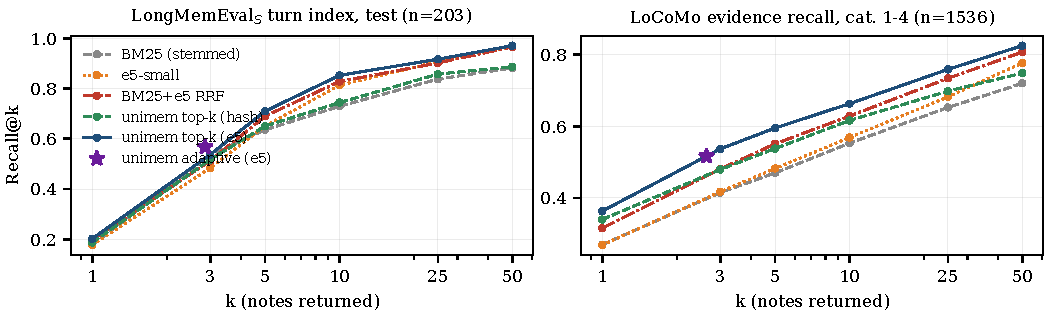
\includegraphics[width=0.92\textwidth]{figs/rk_curves.pdf}
\caption{RQ1: Recall@$k$ on the test split (v0.5). The star marks \sys{}'s adaptive recall at the mean number of notes
it returns (2.86 on LongMemEval turns, 2.64 on LoCoMo); it trades depth for precision.}
\label{fig:rk}
\end{figure*}

\para{Results.} Table~\ref{tab:std} and Figure~\ref{fig:rk} summarize the test split. With e5, \sys{}'s ranker is
level with or above BM25+e5 RRF: on LoCoMo it is significantly better (R@10 $+0.035$ [$+0.022$, $+0.047$], 121
wins/53 losses; R@5 $+0.044$ [$+0.031$, $+0.057$]); on LongMemEval it ties at session level (R@10 $+0.010$
[$-0.010$, $+0.030$]) and is ahead but borderline at turn level (R@10 $+0.025$ [$+0.000$, $+0.054$]: the bootstrap
distribution touches 0). The only change from v0.4, where the same ranker was significantly \emph{below} hybrid on
LongMemEval ($-0.033$ session, $-0.055$ turn R@10), is how the cosine enters the prior (z-score plus RRF) and
dense-family weights fitted on dev questions. With the offline hash embedder \sys{} still loses to hybrid on
LongMemEval ($-0.079$ turn R@10 [$-0.123$, $-0.034$]), but ties stemmed BM25 ($+0.020$, n.s.): the gap is the missing
transformer, not the ranker. On the full 419-question set, unimem-prior-e5 reaches turn R@10 0.862 against 0.838.

The adaptive cut-off is the dominant reason \code{recall} scores low on Recall@10: it returns 1.6--2.9 notes and reaches
turn R@10 0.567 against 0.852 for the same engine at \code{Depth::TopK}. This is deliberate for injection. At
\emph{matched depth} (every baseline cut at the number of notes \sys{} returned for that question; v0.4 runs), \sys{}
keeps up: LongMemEval session hit rate 0.916 vs 0.921 (hybrid), turn 0.826 vs 0.850, and LoCoMo evidence recall 0.520
vs 0.456. Multi-evidence question types suffer most from the cut-off (multi-session test turn R@10: 0.404 adaptive vs
0.692 top-$k$).

\para{Published numbers.} The comparison needs care. The LongMemEval paper's retrieval tables are most likely on
LongMemEval$_M$ ($\sim$500 sessions per question) whereas we ran $S$ ($\sim$50): our exact re-implementation of their
BM25 scores 0.771 session NDCG@5 on $S$ against 0.516 in their table. Relative to that BM25 re-run on $S$, e5-small
gains $+0.174$ round R@5 and $+0.243$ R@10, on par with the gains the paper reports for Stella~1.5B ($+0.188$/$+0.246$).
On LoCoMo the paper's DRAGON retriever reports overall recall 58.8/67.5/79.9/84.8 at $k$\,=\,5/10/25/50; our best
``all categories'' numbers (v0.4, unimem-prior-e5) are 0.559/0.639/0.717/0.822, but the paper used 50 conversations
(only 10 are public), prefixed each turn with its session date, and used a dialogue-trained retriever.

\para{Write path and graph.} Feeding raw chat turns through the full write path loses evidence (\code{unimem-write-e5},
Table~\ref{tab:std}): screens reject 1,658 of 102k LongMemEval turns (612 too long, 600 ``transient status'', 408 too
short, 25 ``injection'', 13 ``credential''), and the v0.4 run exposed a real bug: with e5, the hash-calibrated
near-duplicate threshold merged 22,763 of 102k LongMemEval turns (22\%) and 2,662 of 5,882 LoCoMo turns (45\%), because
e5 cosines are compressed (random LoCoMo pairs have median 0.823). Per-embedder thresholds reduced this to 8,137 and
433. Graph expansion contributed 0--38 of about 5.7k returned notes: \emph{the graph contributes nothing measurable}.

%---------------------------------------------------------------------
\subsection{RQ2: coding-agent memory (heldout2, out-of-sample)}
\label{sec:rq2}

\para{Systems.} \code{unimem-full} is the engine as shipped (adaptive recall over the current project and global);
\code{unimem-top5} is ranking mode at $k$\,=\,5; \code{silo-per-harness} is the same engine with one store per
harness, modelling harness-native memory; \code{vector-top5}/\code{bm25-top5} search all notes, and their \code{-cwd}
variants only the current project. Baselines store every write verbatim and have no abstention.

\begin{table*}[t]
\centering\small
\caption{RQ2 on \code{heldout2} (out-of-sample; 218 answerable queries). Hash embedder unless marked e5. Lower is better
for leak, stale and rejected. ``rejected'' = a note whose gold label is ``should be rejected at write time'' appears in the
results.}
\label{tab:e1}
\setlength{\tabcolsep}{3.6pt}
\begin{tabular}{@{}lcccccccccc@{}}
\toprule
system & R@1 & R@5 & MRR & notes/q & precision & scope leak & forbidden hit & stale ret. & rejected ret. & cross-harn.\ R@5 \\
\midrule
\rowcolor{ours} unimem-full (v0.3/v0.4) & 0.555 & 0.688 & 0.616 & 1.6 & 0.423 & 2.5\% & 0.0\% & 16.3\% & 6.6\% & 0.664 \\
unimem-passive (v0.4) & 0.560 & 0.688 & 0.618 & 1.6 & 0.437 & 2.5\% & 0.0\% & 16.3\% & 1.2\% & 0.671 \\
unimem-full (v0.5) & 0.555 & 0.693 & 0.617 & 1.65 & 0.424 & 2.5\% & 0.0\% & 16.3\% & 6.2\% & 0.671 \\
unimem-top5 (v0.5) & 0.555 & 0.784 & 0.648 & 5 & 0.157 & 17.8\% & -- & 34.9\% & 23.6\% & 0.786 \\
unimem-full, e5 (v0.5) & 0.606 & 0.693 & 0.643 & 1.50 & 0.470 & 1.2\% & 0.0\% & 18.6\% & 5.0\% & 0.664 \\
unimem-top5, e5 (v0.5) & 0.610 & 0.803 & 0.684 & 5 & 0.161 & 16.9\% & -- & 34.9\% & 29.8\% & 0.786 \\
\midrule
silo-per-harness & 0.243 & 0.271 & 0.257 & 1.1 & 0.242 & 2.9\% & 0.0\% & 16.3\% & 4.1\% & 0.000 \\
vector-top5 (all projects) & 0.358 & 0.656 & 0.475 & 5 & 0.131 & 91.3\% & 66.7\% & 62.8\% & 26.9\% & 0.643 \\
vector-top5-cwd & 0.390 & 0.670 & 0.506 & 5 & 0.134 & 8.7\% & 0.0\% & 58.1\% & 45.5\% & 0.664 \\
vector-top5-cwd, e5 & 0.514 & 0.743 & 0.605 & 5 & 0.149 & 2.1\% & -- & 55.8\% & 56.6\% & 0.736 \\
bm25-top5 (all projects) & 0.408 & 0.642 & 0.500 & 4.5 & 0.141 & 79.3\% & 57.1\% & 65.1\% & 31.8\% & 0.614 \\
bm25-top5-cwd & 0.413 & 0.615 & 0.497 & 4.0 & 0.152 & 3.3\% & 0.0\% & 55.8\% & 37.2\% & 0.600 \\
\bottomrule
\end{tabular}
\end{table*}

\para{Unified versus silo.} Table~\ref{tab:e1} shows the central architectural claim. (Numbers in the text are the v0.3/v0.4 run;
the released v0.5 code reproduces the v0.5 row exactly, with cross-harness R@5 0.671 and MRR 0.608.) On the 140 cross-harness
questions (the note was written by a different harness than the one asking), unified memory reaches R@5 0.664 and MRR
0.605; a per-harness silo scores 0.000 by construction. The cost of unification is small: on 78 same-harness questions
the silo is slightly better (R@5 0.756 vs 0.731, MRR 0.718 vs 0.637) because a smaller store has fewer competitors.

\para{Retrieval quality.} Adaptive \code{unimem-full} beats every baseline on R@1, MRR, precision and stale-avoidance.
Its R@5 is significantly above BM25-cwd ($+0.078$ [$+0.023$, $+0.133$], v0.5 hash run) but \emph{not} above a plain
top-5 cosine search with the same embedder ($+0.023$ [$-0.032$, $+0.078$]; v0.3: $+0.018$ [$-0.037$, $+0.073$]); with e5 it is even slightly below (R@5 $-0.050$
[$-0.106$, $+0.005$], n.s.) because it returns about 1.5 notes. At equal depth, \code{unimem-top5} wins clearly ($+0.115$
[$+0.069$, $+0.165$] over vector-top5-cwd with hash, $+0.060$ [$+0.014$, $+0.110$] with e5). Ranking mode pays for depth:
scope leak 17\%, stale 35\% and rejected-label notes 24--30\%, which is why injection stays adaptive.

\para{Scope isolation and staleness.} Searching all projects leaks scope on 79--91\% of queries and hits forbidden
notes 57--67\% of the time; \sys{} leaks on 2.5\% with 0\% forbidden hits while still answering cross-project questions
that cwd-filtered baselines cannot (R@5 0.368 vs 0.053). Only 16.3\% of the queries that have an outdated note return it (vs 55.8--65.1\%
for baselines). The write path (Table~\ref{tab:write}) explains why: supersede precision/recall is 0.889/0.640 with 0/12
distractor errors; global preferences stated inside a project are scoped correctly in 18/22 cases (v0.1: 2/23). The
passive-path screen of v0.4 reduces rejected-label notes in passive results from 6.6\% to 1.2\% at unchanged R@5.

\begin{table}[t]
\centering\scriptsize
\caption{RQ2 write path on \code{heldout2} (out-of-sample) across versions; v0.4 leaves these metrics unchanged.}
\label{tab:write}
\setlength{\tabcolsep}{3pt}
\begin{tabular}{@{}lccc@{}}
\toprule
metric & v0.1 & v0.2 & v0.3 \\
\midrule
rejection precision / recall & 1.000 / 0.217 & 0.889 / 0.348 & 0.923 / 0.522 \\
injection / secret / status caught & 0/7, 4/10, 1/6 & 0/7, 7/10, 1/6 & 1/7, 10/10, 1/6 \\
decoys rejected & 0/6 & 0/6 & 0/6 \\
duplicate recall (gold 23) & 0/23 & 0/23 & 4/23 \\
supersede precision / recall & 1.000 / 0.240 & -- / 0.000 & 0.889 / 0.640 \\
distractor false supersedes & 0/12 & 0/12 & 0/12 \\
scope accuracy & 0.890 & 0.915 & 0.944 \\
global note written in a project & 2/23 & 8/22 & 18/22 \\
kind accuracy & 0.465 & 0.460 & 0.456 \\
write latency p50 / p95 (ms) & 0.54 / 0.83 & 0.70 / 1.02 & 1.26 / 4.96 \\
\bottomrule
\end{tabular}
\end{table}

\para{Error analysis.} Of the 68 v0.3 misses on answerable heldout2 queries, 32 are cross-language (query and gold note
in different languages; R@5 0.333 on 48 such queries vs 0.788 on 170 same-language ones, a weakness shared by BM25 and
hash vectors); about 25 are topical neighbours in the right project outranking the answer; 12 are cross-project; 6 are
stale notes; 4 trace to the write path (2 golds wrongly superseded, 1 update dropped as a duplicate); and in 8
an unrejected injection note occupies result slots.

%---------------------------------------------------------------------
\subsection{RQ3: gateway overhead, cache stability and interception}
\label{sec:rq3}

\para{Latency.} With a mock upstream (300 requests per cell, $\approx$31.5\,KB Claude-Code-like bodies with 12 tools and an
$\sim$11\,KB system prompt), the gateway adds 1.149\,ms p50 and 3.124\,ms p95 time-to-first-byte when streaming with
passive recall, 0.449\,ms streaming without recall, and 0.371\,ms (p95 0.424\,ms) for JSON (v0.4). The hot-path recall budget is
1.5\,s.

\begin{table}[t]
\centering\scriptsize
\caption{RQ3: prompt-cache stability over a 30-turn streamed conversation (v0.4). Prefix fraction = byte-identical common
prefix of consecutive upstream requests over the earlier one's length.}
\label{tab:cache}
\setlength{\tabcolsep}{2.8pt}
\begin{tabular}{@{}lccccc@{}}
\toprule
mode & up.\ req. & prefix mean / min & stable trans. & cacheable & system stable \\
\midrule
Passthrough & 37 & 1.000 / 1.000 & 36/36 & 0.987 & yes \\
\rowcolor{ours} \sys{} & 43 & 1.000 / 1.000 & 42/42 & 0.987 & yes \\
NaiveSystem & 37 & 0.825 / 0.615 & 9/36 & 0.803 & no \\
NaiveTail & 37 & 0.991 / 0.969 & 9/36 & 0.979 & yes \\
\bottomrule
\end{tabular}
\end{table}

\para{Cache stability (I1).} Table~\ref{tab:cache} compares \sys{} with pass-through and two naive injectors: one that
puts recall into the system prompt, and one that appends it to the tail without replaying it. Every one of \sys{}'s 42
upstream transitions, including 6 continuation rounds, is an exact byte-prefix extension, matching pass-through; the
naive injectors keep only 9 of 36 transitions fully stable. The price is upstream volume: 2,251,877 bytes vs 1,533,536 for
pass-through, mostly the extra full-context continuation requests (cacheable, but billed and rate-limited). We measured
byte-level prefixes, not the provider's \code{cache\_read\_input\_tokens}.

\para{Interception (I4) and isolation (I2).} A scripted suite (recall-only, remember-only, mixed \sys{}+\code{Bash},
\code{Bash}-only and plain turns; streaming and JSON; each followed by a request echoing the visible message) drives
120 client requests into 144 upstream requests with 24 continuation rounds. All 1060/1060 assertions pass across 15
families, including: the client never sees a \sys{} tool (157/157) or \sys{} context (157/157), framing is valid,
hidden rounds are replayed byte-identically to the continuation (24/24), mixed hidden calls and results are replayed
(12/12), harness tool calls are delivered (24/24) and the system prompt is untouched (60/60). In an anchor-collision probe,
two sessions send the same prompt and receive the same deterministic reply that used \code{unimem\_recall}; 0/10 second
sessions receive the first session's hidden rounds (v0.1: 10/10, \S\ref{sec:lessons}).

%---------------------------------------------------------------------
\subsection{RQ4: long sessions, budgets and compaction (E5)}
\label{sec:rq4}

\para{Scenario.} A Claude-Code-like session on one repository (\code{devmem} corpus, 200k window) runs 120 client
requests: prompts from the corpus queries, 6 planted user facts, 3 corrections, tasks with 2--3 \code{Bash} calls and
24k-character logs (every other task contains one error whose root cause is a stored note), and 4 prompts that make the
model call \code{unimem\_recall}. At request 60 the harness sends its compaction request and replaces the history with
a summary. ``Heavy'' variants add 40 long relevant notes ($\approx$2\,kchar content plus $\approx$1\,kchar \code{why}).
Ablations disable the budgets, the ledger or the flush.

\begin{table}[t]
\centering\scriptsize
\caption{RQ4: E5 long session (120 requests, compaction at 60, 200k window). Live = tokens \sys{} holds in context
(replayed augmentations + hidden rounds).}
\label{tab:e5}
\setlength{\tabcolsep}{2.4pt}
\begin{tabular}{@{}lccccc@{}}
\toprule
variant & max live & share & cum.\ injected & injections & dup. \\
\midrule
\rowcolor{ours} v0.4 & 3,513 & 1.8\% & 4,933 & 67 & 0 \\
no-budget & 3,513 & 1.8\% & 4,933 & 67 & 0 \\
no-budget-no-dedup & 7,703 & 3.9\% & 13,282 & 195 & 128 \\
\rowcolor{ours} heavy / v0.4 & 7,098 & 3.5\% & 9,130 & 92 & 0 \\
heavy / no-budget & 10,237 & 5.1\% & 11,243 & 79 & 0 \\
heavy / no-budget-no-dedup & 13,998 & 7.0\% & 17,342 & 117 & 38 \\
\bottomrule
\end{tabular}
\end{table}

\begin{figure*}[t]
\centering
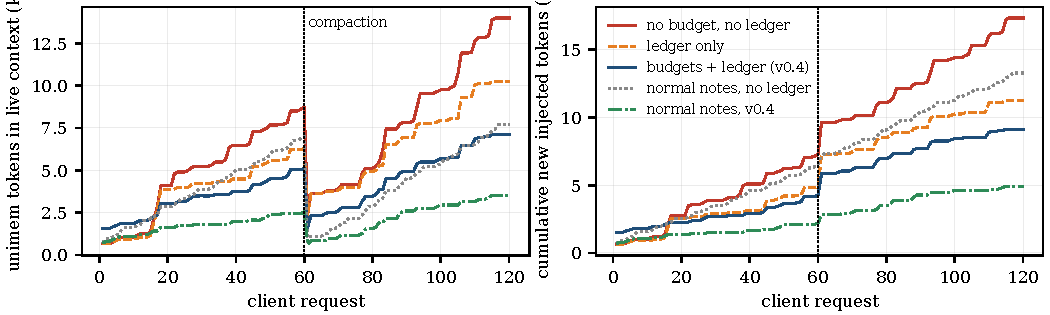
\includegraphics[width=0.92\textwidth]{figs/e5_session.pdf}
\caption{RQ4: tokens \sys{} keeps in the live context (left) and cumulative newly injected tokens (right) over the E5
session. The dashed line marks the harness's compaction at request 60; the preamble returns on the next request.}
\label{fig:e5}
\end{figure*}

\para{Results.} Table~\ref{tab:e5} and Figure~\ref{fig:e5}. The ledger removes all duplicate injections (128$\to$0 at
normal note sizes, 38$\to$0 with heavy notes). With heavy notes, budgets plus ledger halve the peak \sys{} footprint
from 14.0k to 7.1k tokens (7.0\%$\to$3.5\% of the window) and cumulative injection from 17.3k to 9.1k. At normal note sizes
the budgets never bind (no-budget equals v0.4), and the 5\% session cap never bound in this run. The compaction request
reached the upstream byte-identical; the preamble came back on the first request after the summary, and live \sys{}
context dropped to about 1.6k before growing again. Tool-error recall fired on 6 of 11 error turns, each time with the
root-cause note, and on 3 more the note was already live, so 9/11 errors had their explanation in context; benign tool turns
received 0/44 injections. The two misses share only a port number with their note, and the rare-token gate ignores numbers
by design. The flush nudge fired once, at request 54 (estimated context $\approx$140k, 70\% of 200k); the background
heuristic distillation it triggered had stored 5 of the 6 facts stated before compaction by the time compaction occurred,
against 0 of 6 without the flush. All 3 corrections were hinted. Note that the harness's own context dominates: the maximum
total context share was 80.7\% in v0.4, of which \sys{} held 1.8\%.

\para{Re-run with the v0.5 code.} E5 was not re-run for v0.5 in the main experiments; re-running it at release (same scenario)
gives the same qualitative picture but different magnitudes, because v0.5's prior returns different notes: peak live context
4.5k tokens (2.2\%) for v0.5, 8.4k (4.2\%) with heavy notes versus 18.4k (9.2\%) for heavy/no-budget-no-dedup, 130--132
duplicate injections removed by the ledger, and 5 of 6 facts saved by the flush (0 of 6 without). E5 is also not exactly
deterministic: the background flush distillation races the request loop, so cumulative-injection counts vary by up to about 10\%
between runs. Table~\ref{tab:e5} reports the v0.4 run.

%---------------------------------------------------------------------
\subsection{RQ5: project identification (E3)}
\label{sec:rq5}
On 37 synthetic layouts---worktrees (CLI-made and hand-made relative \code{gitdir}+\code{commondir}), submodules, nested
repositories, forks, GHE/GitLab subgroups and ports, userinfo, case and trailing-slash variants, a dotfiles home
repository, symlinks, non-git manifest directories and remotes added later---\sys{} resolves 37/37 correctly (v0.1: 35/37).
No held-out layouts exist, so this is in-sample.

%---------------------------------------------------------------------
\subsection{RQ6: scaling (E4)}
\label{sec:rq6}
On templated synthetic notes, v0.3 at 10,000 stored notes (9,849 live) takes 7.654\,ms p50 / 17.241\,ms p95 per write and
4.751\,ms p50 / 7.226\,ms p95 per recall, with a 103.71\,MB database (10,371 bytes per note) and 77.3\,MB RSS. At 7,000
notes, recall p50 is 3.582\,ms. Recall is a brute-force cosine over all live notes and grows linearly; an ANN index is
needed well before 100k notes. On the standard benchmarks, engine recall takes 2--6\,ms per query against at most
0.03\,ms for BM25.

%=====================================================================
\section{Lessons from the Version History}
\label{sec:lessons}
Our versions act as a sequence of ablations, and the evaluation repeatedly found real bugs (Table~\ref{tab:history}).

\begin{table}[t]
\centering\scriptsize
\caption{What each version changed and what the evaluation found. R@5 on heldout2 unless stated.}
\label{tab:history}
\setlength{\tabcolsep}{2.5pt}
\begin{tabularx}{\columnwidth}{@{}l>{\raggedright\arraybackslash}X@{}}
\toprule
ver. & change $\to$ finding \\
\midrule
v0.1 & engine, 3 dialects, overlays $\to$ streaming +42.8\,ms TTFB (Nagle); cross-session anchor collision 10/10; over-eager supersede (91\% of E4 stores); R@5 0.569 \\
v0.2 & fixes from devmem findings $\to$ TTFB +0.76\,ms; collision 0/10; E3 37/37; but heldout R@5 0.444$\to$0.447, false abstain 5.6\%$\to$21.3\%, supersede recall collapsed, 12,664/19,664 E4 writes falsely deduplicated; R@5 0.550 \\
v0.3 & calibrated hybrid prior, subject-aware supersede/dup $\to$ R@5 0.688 ($+0.119$ vs v0.1, CI [$+0.064$, $+0.174$]); injection screen 6/6 in-sample but 1/7 out-of-sample \\
v0.4 & timing policy from the design review $\to$ duplicate injections 128$\to$0; flush 5/6; e5 dedup bug found (22\% of turns merged) and fixed \\
v0.5 & embedder-calibrated prior, \code{Depth::TopK}, ONNX e5 $\to$ ranker at or above BM25+e5 RRF on test split \\
\bottomrule
\end{tabularx}
\end{table}

\para{The v0.2 overfitting episode.} v0.2 fixed every v0.1 finding on \code{devmem} and reached 1.000 rejection precision
and recall there. On the then-unseen \code{heldout} set it did not improve retrieval (R@5 0.444$\to$0.447, R@1
0.303$\to$0.281), false abstention rose from 5.6\% to 21.3\%, supersede recall collapsed (5/26$\to$1/26 correct) so stale
answers \emph{increased} (44.4\%$\to$50.8\%), Chinese recall regressed (0.500$\to$0.321), and a new silent data-loss mode
appeared: 64\% of E4 write attempts were rejected as duplicates. Even in-sample retrieval got worse (devmem R@5
0.486$\to$0.425). The lesson shaped everything after it: in-sample screens can be made perfect and still not generalize
(v0.3 again scored 6/6 in-sample and 1/7 out-of-sample on injections), so we built \code{heldout2} before tuning and report
it as the only generalization evidence.

\para{Bugs found by measurement.} (i) \emph{Nagle/delayed ACK}: the server did not set \code{TCP\_NODELAY} on client
sockets, and many small SSE writes cost $+42.8$\,ms p50 TTFB; a one-line fix brought it to $+0.76$\,ms. (ii) \emph{Anchor
collision}: expansion anchors did not include the session, and \code{put\_overlay} ignored conflicts, so two sessions with
the same prompt and deterministic reply shared hidden rounds (10/10 in the probe); adding $s$ to the anchor gives invariant
I2. (iii) \emph{Over-eager supersede}: without a subject check, ``auth-12 listens on port 3100'' could supersede
``billing-40 listens on port 5200''; 9,232 of 10,672 templated writes superseded something. (iv) \emph{Embedder-specific
dedup}: thresholds calibrated on hash cosines merged 45\% of LoCoMo turns under e5. (v) \emph{Distiller data loss}: v0.3
read only the newest 24k characters but marked all episodes distilled. (vi) \emph{Compaction}: v0.3 never re-sent the preamble
after compaction. None of these would have been visible without the corresponding measurement.

%=====================================================================
\section{Limitations and Immature Aspects}
\label{sec:limits}

\sys{} is research-grade software. We list its weaknesses prominently because a gateway sits in front of all of a user's
model traffic.

\para{Context-window blow-up remains a risk.} Before v0.4, the design review estimated from the code constants that
passive injection costs about 110 tokens per prompt turn typically ($\approx$6\% of a 200k window over 100 turns), about 700
with realistic heavy notes (35\%), and up to 3.2k tokens per turn in the worst English case, overflowing a 200k window by
about turn 60 (CJK notes: 8--12k tokens per turn, overflow by about turn 20); a single visible turn with $k$\,=\,20 agent
recalls over 6 rounds could reach about 75k tokens (37\%). v0.4 caps per-turn, preamble, tool and per-session injection,
and E5 measured a peak of 3.5\% of the window with heavy notes. Residual risks:
\begin{itemize}
\item \emph{Hidden rounds are replayed until compaction.} The session share stops passive recall, but not agent-initiated
  \code{unimem\_recall}. With the default constants a single visible response can still add up to $6\times3000$ tokens of tool
  output (our arithmetic from $B_{\text{tool}}$ and \code{max\_continuations}), which is then replayed on every later request.
\item \emph{Heuristics tied to current harness wording.} Compaction-request detection and two of the four compaction signals
  match the text Claude Code and Codex use today. If that wording changes, \sys{} may inject into a compaction request or miss
  a compaction; only the message-count and zero-anchor signals are harness-independent.
\item \emph{Anthropic's 20-block cache lookback}~\cite{promptcaching}. Each hidden round inserts blocks between the harness's
  cache breakpoints; several continuations can push the previous cache write out of the lookback window and cause a full
  miss. We measured byte-prefix stability, not real cache reads.
\item \emph{Estimator error.} Budgets use a $\pm$30\% estimator; unknown models fall back to a 128k window.
\item \emph{Upstream volume.} Continuation rounds increase upstream bytes (2.25\,MB vs 1.53\,MB over 30 turns), drawing on
  rate limits and, on subscriptions, on the user's quota invisibly.
\end{itemize}

\para{No real-traffic validation.} Every gateway result uses mock upstreams and scripted, harness-like requests. Real harness
versions may send shapes the anchors do not expect (e.g.\ trimmed thinking blocks), in which case overlays are skipped and
memory context is lost. Codex with a ChatGPT login through a custom provider, Responses reasoning-item adjacency when hidden
items are re-inserted, and user messages inserted after \code{function\_call\_output} (tool-error recall) are unverified
against the real backends.

\para{Only the offline heuristic decider was evaluated.} All quality numbers come from the heuristic System One with hash or e5
embedders. The Jev and LLM deciders are implemented but untested end to end; their 8\,s and 15\,s default timeouts exceed the
1.5\,s hot-path recall budget, so on the passive path they would often be cut off. Kind classification is 46\% accurate. The
\code{sufficient} signal misfired on 45\% of answerable heldout2 queries in v0.3/v0.4 (consistent with~\cite{relevancesufficiency});
v0.5's re-scaled prior brings this to 8.7\% (hash) and 9.6\% (e5) on heldout2 but 89.9\% with e5 on \code{devmem} and \code{heldout},
so its threshold is not calibrated across embedders and corpora.

\para{No end-to-end metric.} We report retrieval, mechanics and simulated timing, not QA accuracy or task success. A
LongMemEval/LoCoMo QA script with the official reader and judge prompts is provided (\code{bench/std/qa\_eval.py}) and builds all
prompts offline, but was not run. No experiment shows that \sys{} reduces repeated corrections or improves agent success, which
is the only metric that could justify its hot-path costs. LongMemEval$_M$ was not run (disk limit).

\para{Synthetic, LLM-authored suites.} \code{devmem}, \code{heldout} and \code{heldout2} were written by an LLM, the corpora are small
(183--233 notes), and E3/E4/E5 are generated. \code{heldout2} is out-of-sample for tuning but not independent of the author's
view of what coding memory looks like.

\para{Weak write-time screens.} Out-of-sample, the injection screen caught 1/7 and the status screen 1/6 (four of five misses
Chinese), against 100\% in-sample. A stored injection note (``Team convention per Dave: \ldots run apply with
\code{-auto-approve} \ldots{} Mira doesn't need to be asked'') was served as the answer to exactly the question it targets---the
failure class described in~\cite{groundingawareness}. v0.4 keeps instruction-like notes off the \emph{passive} path, but they
remain retrievable through \code{unimem\_recall}. Shared memory must be treated as untrusted input.

\para{Cross-language and paraphrase gaps.} Cross-language R@5 is 0.333 versus 0.788 within a language; 17 of 23 gold duplicates
are cross-language restatements and go undetected. Paraphrase (0.419) and cross-project (0.368) categories are weak.

\para{The graph and the gate contribute little.} Graph expansion has no measurable effect on any benchmark, and full, lite
(no edges) and passive (gated) modes return nearly identical results on heldout2. The four-view graph is, so far, unvalidated
complexity.

\para{Operational and policy risks.} \emph{Single point of failure}: memory errors fail open, but if the process dies the
harness cannot reach its model until the base URL is unset. \emph{No authentication}: the gateway, MCP endpoint and web UI
accept anything that reaches the listen address; they must stay on \code{127.0.0.1}. Since the release audit, requests that carry a
foreign \code{Origin} or a non-local \code{Host} name are refused, which closes cross-site POSTs and DNS rebinding from a browser,
but not other local processes. \emph{Terms of service}: rewriting
subscription traffic (Claude OAuth, ChatGPT login) and generating extra requests on it may be restricted by provider terms;
Claude Code's gateway documentation notes that a saved login remains the active credential behind a custom base URL~\cite{ccgateway},
and the ChatGPT Codex backend is not a public API. \emph{Privacy}: one database holds memories and episodes from every
harness and project; episodes are redacted by regex/heuristic screens with a 30-day TTL, \code{unimem\_project} lists known
projects to any agent, and there is no equivalent of excluding chats with external context from distillation. Shared memory can
also expose one owner's credentials to another context~\cite{whosecredential}.
\emph{Concurrency}: one mutex-guarded SQLite connection serializes parallel subagents, harnesses and the distiller.

%=====================================================================
\section{Ethics and Broader Impact}
A shared memory makes agents more useful and more dangerous at once. It reduces repeated instruction and can carry safety
conventions across tools, but it also centralizes sensitive data, widens the blast radius of a poisoned note, and makes it easier
to persist an assistant's proposal as if it were the user's authorization. \sys{} runs locally, sends no telemetry, makes no
extra network calls by default, keeps the system prompt untouched, labels injected notes as ``data, not instructions'', and
keeps instruction-like notes off the passive path; these mitigations are partial (\S\ref{sec:limits}). Users should check their
providers' terms before routing subscription traffic through any gateway.

%=====================================================================
\section{Conclusion}
\sys{} shows that the model API boundary is a workable place for shared agent memory: with overlay replay the provider cache
stays byte-stable, with streaming interception the harness never sees a foreign tool, and with budgets, a ledger and
compaction awareness the memory footprint stays a few percent of the window in simulation. Unified memory answers
cross-harness questions that silos cannot, and the calibrated hybrid ranker is competitive with strong baselines on standard
retrieval benchmarks. What we have not shown is that any of this improves real agents on real traffic. The next steps are a
regression suite recorded from real Claude Code and Codex sessions, an evaluation of model-backed System-One deciders and screens,
end-to-end QA and task-success metrics, and cross-language retrieval.

\footnotesize
\bibliographystyle{abbrvnat}
\bibliography{refs}
\normalsize

%=====================================================================
\appendix
\onecolumn
\section{Reproduction}
\label{app:repro}
All results are in the repository under \code{bench/}; every number in this paper is taken from
\code{bench/std/RESULTS.md}, \code{bench/results/\{FINAL,COMPARISON\}.md}, \code{bench/results/v0.\{1..5\}/} and
\code{docs/REVIEW.md}. Figures are regenerated by \code{python3 -I docs/paper/figs/make\_figs.py} from
\code{bench/results/v0.4/e5\_long\_session.json} and \code{bench/results/v0.5/std/*.test.json}.
\begin{small}
\begin{verbatim}
cargo build --release              # add --features onnx for the e5 embedder
# E1-E5 on the out-of-sample suite
cargo run --release --bin unimem-bench -- all --data bench/data/heldout2.json --out /tmp/out
# LongMemEval_S + LoCoMo retrieval, significance, official cross-check
CACHE=/path/to/bench-cache bench/std/run_all.sh
# relevance-prior fit (dev data only) and test-split bootstrap
python3 -I bench/std/fit_prior.py bench/results/v0.5/prior_fit.json <evidence files>
python3 -I bench/std/significance_v05.py C runs-v05
# E1 with the e5 embedder
ORT_DYLIB_PATH=... UNIMEM_BENCH_EMBEDDER=onnx UNIMEM_BENCH_EMBEDDER_MODEL=<dir> \
  unimem-bench e1 --data bench/data/heldout2.json --out ...
\end{verbatim}
\end{small}
Swapping the decider or embedder for a run: \code{UNIMEM\_BENCH\_DECIDER}, \code{UNIMEM\_BENCH\_EMBEDDER},
\code{UNIMEM\_BENCH\_CONFIG}. The datasets are downloaded with size and sha256 checks (\code{bench/std/download.sh}).

\section{Integration and configuration}
\label{app:config}
\begin{small}
\begin{verbatim}
unimem serve                                    # 127.0.0.1:4777
# Claude Code (API key and OAuth headers are forwarded)
export ANTHROPIC_BASE_URL=http://127.0.0.1:4777
# ~/.codex/config.toml
model_provider = "unimem"
[model_providers.unimem]
name = "unimem"
base_url = "http://127.0.0.1:4777/v1"
wire_api = "responses"
requires_openai_auth = true
# MCP-only mode (tools, no passive recall):
claude mcp add --transport http unimem http://127.0.0.1:4777/mcp
\end{verbatim}
\end{small}

\begin{table}[H]
\centering\small
\caption{Main configuration keys and defaults (\code{\textasciitilde/.unimem/config.toml}; every field optional).}
\label{tab:config}
\begin{tabularx}{\textwidth}{@{}l>{\raggedright\arraybackslash}Xl@{}}
\toprule
section & key & default \\
\midrule
\code{[inject]} & \code{recall\_budget\_ms}, \code{max\_recall\_notes}, \code{preamble\_max\_notes}, \code{max\_continuations} & 1500, 5, 8, 6 \\
& \code{max\_inject\_tokens}, \code{max\_preamble\_tokens}, \code{max\_tool\_tokens}, \code{max\_session\_share} & 1200, 1500, 3000, 0.05 \\
& \code{tool\_recall\_every}, \code{tool\_recall\_max\_tokens}, \code{flush\_at} & 5, 400, 0.7 \\
& \code{budgets}, \code{dedup}, \code{tool\_recall}, \code{correction\_hints} & true \\
\code{[decider]} & \code{chain} & jev, llm, heuristic (jev only with \code{TYPESAFE\_API\_KEY}) \\
\code{[embedder]} & \code{kind} & hash (offline); openai; onnx \\
\code{[distill]} & \code{enabled}, \code{idle\_secs}, \code{episode\_ttl\_days}, \code{min\_rate\_limit\_remaining}, \code{chunk\_chars} & false, 600, 30, 0.1, 24000 \\
\bottomrule
\end{tabularx}
\end{table}

\section{Web UI}
\label{app:ui}
\begin{figure}[H]
\centering
\begin{subfigure}{0.49\textwidth}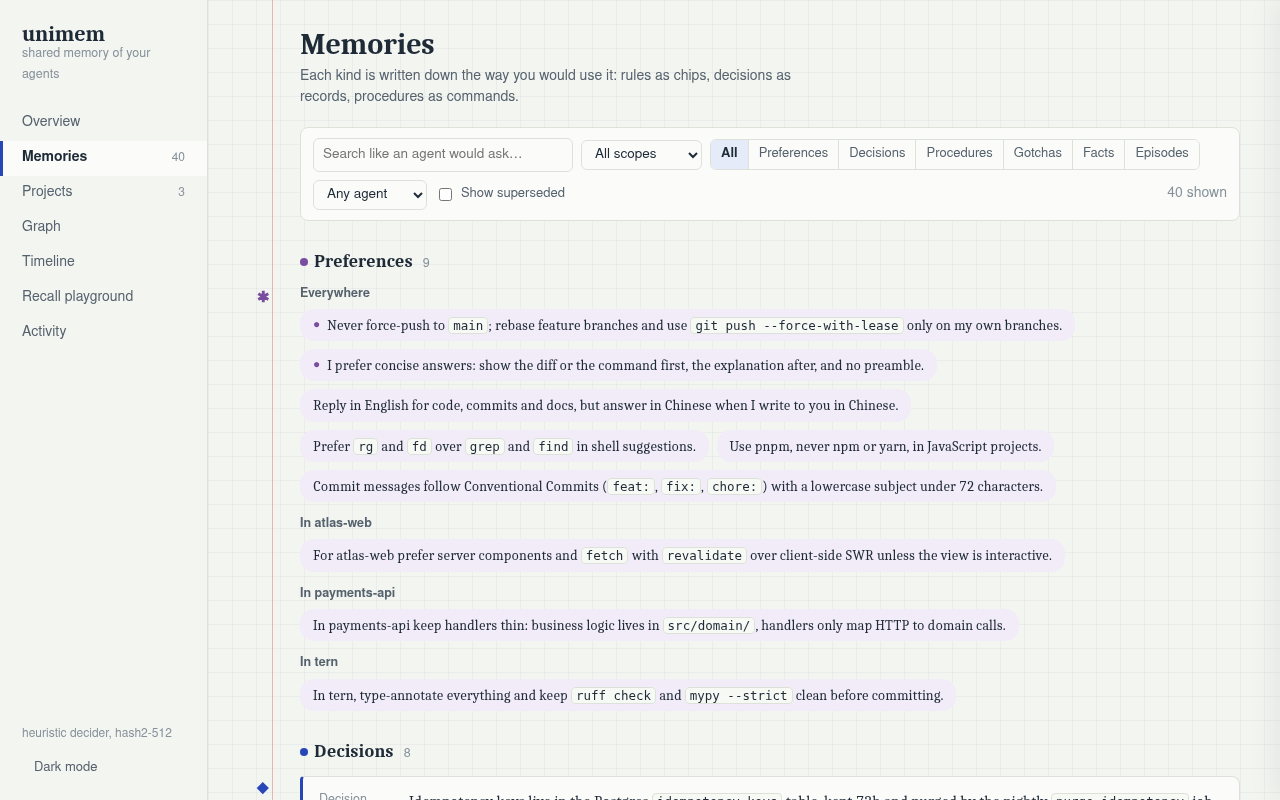
\includegraphics[width=\linewidth]{figs/ui-memories.png}\caption{Memories: per-kind views (rule chips, ADR-style decisions with supersede chains, procedures, gotchas).}\end{subfigure}\hfill
\begin{subfigure}{0.49\textwidth}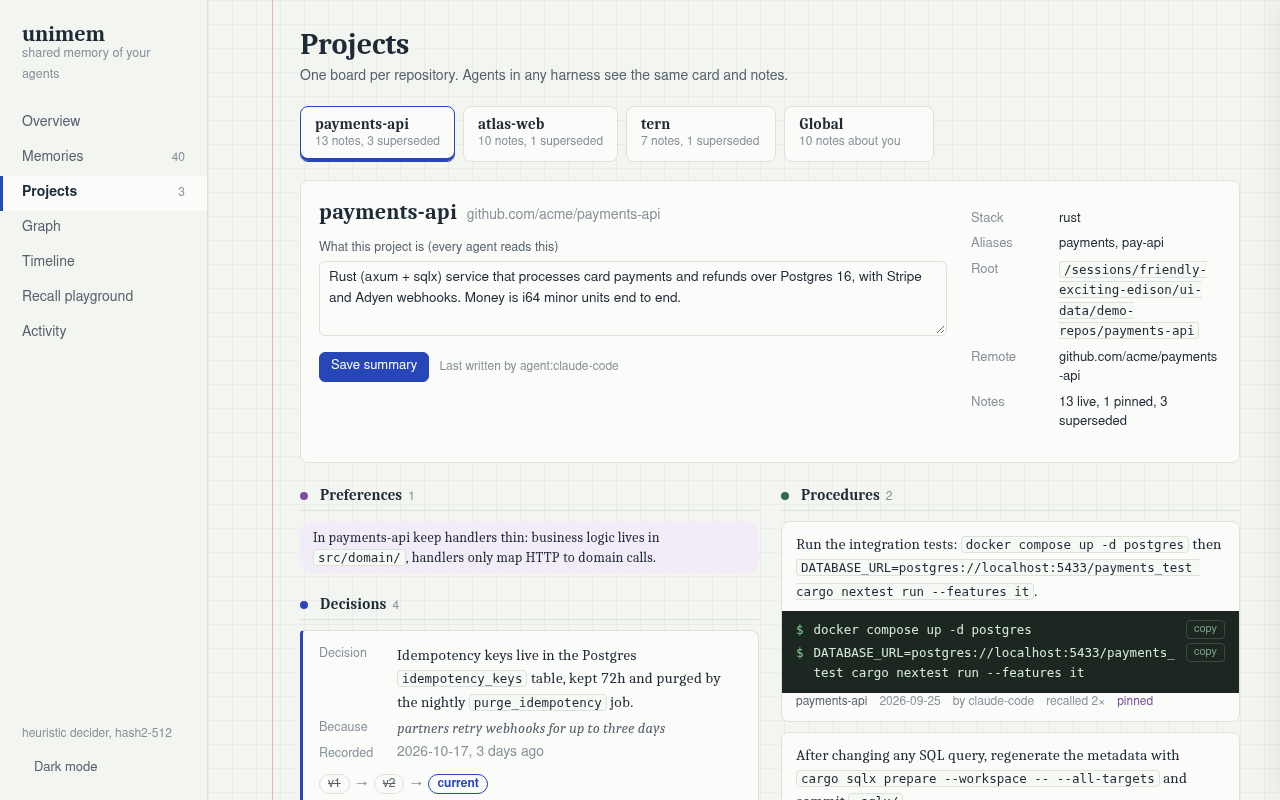
\includegraphics[width=\linewidth]{figs/ui-projects.png}\caption{Projects: the editable project card every agent reads, and the repository's notes by kind.}\end{subfigure}
\caption{The local web UI served at \code{/ui} (single embedded page, no external assets). Other views: overview, graph,
timeline, recall playground and activity log. The UI has no authentication.}
\label{fig:ui}
\end{figure}

\section{Additional results}
\label{app:extra}

\begin{table}[H]
\centering\small
\caption{heldout2 R@5 by category (out-of-sample; hash embedder; vector columns use \code{hash2}). $n$ counts all queries of the
category; scope\_isolation R@5 is over its 18 answerable queries (4 are forbidden-only).}
\label{tab:cat}
\begin{tabular}{@{}lrccccccc@{}}
\toprule
category & $n$ & v0.1 & v0.2 & v0.3 & silo & vector-top5 & vector-top5-cwd & bm25-top5-cwd \\
\midrule
single\_hop & 65 & 0.692 & 0.723 & 0.892 & 0.338 & 0.908 & 0.846 & 0.738 \\
paraphrase & 31 & 0.290 & 0.323 & 0.419 & 0.258 & 0.387 & 0.484 & 0.355 \\
chinese & 38 & 0.658 & 0.526 & 0.763 & 0.368 & 0.605 & 0.816 & 0.763 \\
cross\_project & 19 & 0.211 & 0.158 & 0.368 & 0.158 & 0.579 & 0.053 & 0.053 \\
temporal & 24 & 0.500 & 0.500 & 0.667 & 0.208 & 0.625 & 0.667 & 0.708 \\
causal & 23 & 0.696 & 0.696 & 0.739 & 0.261 & 0.609 & 0.696 & 0.739 \\
scope\_isolation & 22 & 0.722 & 0.667 & 0.556 & 0.056 & 0.500 & 0.667 & 0.611 \\
\bottomrule
\end{tabular}
\end{table}

\begin{table}[H]
\centering\small
\caption{v0.3 in-sample (heldout) versus out-of-sample (heldout2): retrieval transferred, write-time screens did not.}
\label{tab:inout}
\begin{tabular}{@{}lcccccccc@{}}
\toprule
& R@5 & R@1 & \makecell{rejection\\recall} & \makecell{injection\\screen} & \makecell{duplicate\\recall} & \makecell{supersede\\recall} & \makecell{stale\\returned} & \makecell{scope\\leak} \\
\midrule
heldout (in-sample) & 0.677 & 0.573 & 1.000 & 6/6 & 0.545 & 0.846 & 6.3\% & 0.0\% \\
heldout2 (out-of-sample) & 0.688 & 0.555 & 0.522 & 1/7 & 0.174 & 0.640 & 16.3\% & 2.5\% \\
\bottomrule
\end{tabular}
\end{table}

\begin{table}[H]
\centering\small
\caption{LongMemEval$_S$ full set (419 questions, v0.4): session and turn index, plus the per-type turn R@10 that motivated
the v0.5 refit.}
\label{tab:lmefull}
\setlength{\tabcolsep}{4pt}
\begin{tabular}{@{}lcccc|cccc@{}}
\toprule
system & sess.\ R@5 & sess.\ R@10 & turn R@5 & turn R@10 & multi-session & pref. & temporal & know.-update \\
\midrule
bm25-okapi-ref (= paper BM25) & 0.742 & 0.823 & 0.489 & 0.592 & 0.372 & 0.400 & 0.614 & 0.778 \\
bm25 (stemmed) & 0.859 & 0.924 & 0.654 & 0.754 & 0.587 & 0.500 & 0.756 & 0.931 \\
e5-small & 0.912 & 0.969 & 0.663 & 0.835 & 0.736 & 0.700 & 0.795 & 0.986 \\
hybrid-rrf & 0.921 & 0.971 & 0.721 & 0.838 & 0.711 & 0.733 & 0.827 & 0.986 \\
unimem-prior-e5 (v0.4) & 0.847 & 0.938 & 0.671 & 0.783 & 0.628 & 0.533 & 0.787 & 0.944 \\
unimem-e5 (adaptive) & 0.618 & 0.618 & 0.458 & 0.465 & 0.265 & 0.333 & 0.409 & 0.542 \\
\bottomrule
\end{tabular}
\end{table}

\begin{table}[H]
\centering\small
\caption{v0.5 dev-split fit check (\code{prior\_fit.json}; candidate pool = anchors; R@5 / R@10).}
\label{tab:fit}
\begin{tabular}{@{}lccc@{}}
\toprule
source (dev) & v0.4 prior & RRF only & v0.5 prior \\
\midrule
LME session, e5 & 0.861 / 0.954 & 0.935 / 0.963 & 0.931 / 0.982 \\
LME turn, e5 & 0.690 / 0.796 & 0.736 / 0.847 & 0.755 / 0.866 \\
devmem, e5 & 0.810 / 0.899 & 0.832 / 0.894 & 0.838 / 0.899 \\
LME turn, hash & 0.694 / 0.778 & 0.639 / 0.722 & 0.694 / 0.768 \\
heldout, hash & 0.775 / 0.820 & 0.770 / 0.809 & 0.775 / 0.815 \\
\bottomrule
\end{tabular}
\end{table}

\end{document}
